\documentclass{beamer}

%Podemos usar los diferentes temas
%\usetheme{Goettingen}
%\usetheme{Berkeley}
%Transparencias ugr --> Boadilla
%\usetheme{Boadilla}
%\usetheme{Copenhagen}

\usepackage[utf8]{inputenc}
\usepackage[spanish]{babel}
\usepackage{ dsfont }
\usepackage{mathrsfs}
\usepackage{multimedia}
\usepackage{ocgx2}
\usepackage{media9}
\usepackage{tikz}
\usepackage{graphicx}
\usetheme{CambridgeUS}


\let\emph\relax
\newcommand{\emph}{\alert}

%en corchetes ponemos nombres más cortos, para mejor visualización de las cabeceras del documento
\title[Entendiendo teoría de nudos]{Entendiendo la teoría de nudos mediante la simulación y la informática gráfica.}
\subtitle{Trabajo Fin de Grado}
\date{\today}
\author[Cristina Zuheros]{Cristina Zuheros Montes}
\institute[UGR]{Universidad de Granada.\\
	            \textbf{Tutores:}\\
				Antonio Martínez López. \\
				Alejandro J. León Salas.}

\begin{document}


\maketitle

\begin{frame}{Tabla de contenidos.}
	\setbeamertemplate{section in toc}[sections numbered]
	\tableofcontents[hideallsubsections]
\end{frame}
\AtBeginSection{ 
	\begin{frame} 
		\frametitle{Índice}
		\tableofcontents[currentsection]
	\end{frame}
}
\section{Teoría de nudos.}
\begin{frame}{Definición de nudo (I).}
		\begin{block}{\textbf{\emph{Nudo}}}
			Curva cerrada en $\mathds{R}^{3}$ que no tiene auto-intersecciones.
		\end{block}
	   \begin{figure}[h!]
	   	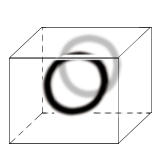
\includegraphics[width=3cm]{imagenes/cubo1.png}
	   	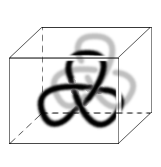
\includegraphics[width=3cm]{imagenes/cubo2.png} 
	   	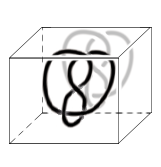
\includegraphics[width=3cm]{imagenes/cubo3.png} 
	   	\centering
	   \end{figure}
	 
	 \pause 
	 Dos nudos son equivalentes si existe un homeomorfismo de  $\mathds{R}^{3}$ que nos lleve de un nudo al otro. \\

\end{frame}

\begin{frame}{Definición de nudo (II).}
	Podemos representar un nudo en el plano visualizando su proyección. Obtenemos una serie de cruces. 
		 \begin{figure}[h!]
		 	
\includegraphics[width=2cm]{imagenes/1.jpg} 
		 	
\includegraphics[width=2cm]{imagenes/3f.png}
		 	
\includegraphics[width=2cm]{imagenes/fig8.jpg}
		 	\centering 
		 \end{figure}
    \pause
	Un \textbf{\emph{enlace}} es una o más curvas cerradas disjuntas en $\mathds{R}^{3}$. Cada curvas es una componente.
		 \begin{figure}[h!]
		  	
\includegraphics[width=2.7cm]{imagenes/enlace.png}
		 \end{figure}
\end{frame}

\begin{frame}{Historia y aplicaciones.}
	\begin{itemize}
		\item Surge hace poco más de 200 años:\\
		Objetivo: crear tabla de nudos que reemplazaría la tabla periódica.
		\item Numerosas cuestiones abiertas:
		\begin{itemize}
			\item Nudos de n-cruces.
			\item Unkotting number.
			\item Crossing number.
			\item Equivalencia de nudos.
			\item Dada una proyección, estudiar trivialidad. 
		\end{itemize}
		\item Aplicaciones en:
		\begin{itemize}
			\item Biología: estructura ADN. 
			\item Criptografía: se aplica teoría de trenzas. 
		\end{itemize}
	\end{itemize}
\end{frame}

\begin{frame}{Composición de nudos (I).}
	Sean J y K proyecciones de nudos. \\
	\begin{figure}[h!]
		
\includegraphics[width=2cm]{imagenes/conexion1.jpg}
		
\includegraphics[width=2cm]{imagenes/fig8.jpg}
	\end{figure}
	\begin{block}{\textbf{\emph{Suma conexa}} \textbf{J\#K}}
		Nudo que obtenemos eliminando un arco de cada proyección y conectando los extremos finales mediante arcos sin añadir ni eliminar cruces.
	\end{block}
	\begin{figure}[h!]
		
\includegraphics[width=5cm]{imagenes/conexion3.jpg}
	\end{figure}
\end{frame}

\begin{frame}{Composición de nudos (II).}
	\begin{itemize}
		\item \textbf{\emph{Nudo primo}}: no puede ser expresado como la suma conexa de dos nudos (salvo factor nudo trivial). 
		\item \textbf{\emph{Nudo compuesto}}: no es el nudo trivial ni es un nudo primo.
		\item \textbf{\emph{Nudo orientado}}: nudo que dispone de una dirección de viaje sobre él mismo. Se indica mediante flechas en la proyección. 
		\item \textbf{\emph{Nudo invertible}}: nudo que es equivalente a sí mismo con la orientación opuesta. \\
	\end{itemize}
\begin{figure}[h!]
	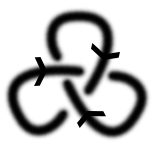
\includegraphics[width=2cm]{imagenes/3fcon1.png}
	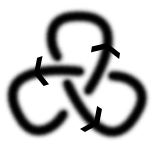
\includegraphics[width=2cm]{imagenes/3fcon2.png}
\end{figure}
\end{frame}

\begin{frame}{Equivalencia de nudos (I).} 
    \begin{alertblock}{\begin{center}
    			\textbf{Teorema de Reidemeister}
    		\end{center}}
    	\begin{center}
    		Sean P1 y P2 las proyecciones que representan a dos nudos K1 y K2, respectivamente. Entonces, K1 $\thicksim$ K2 $\leftrightarrow$ P1 y P2 están conectados por una secuencia finita de isotopías planas y movimientos de Reidemeister.
    	\end{center}
    \end{alertblock}
    \vspace{1cm}
    \pause
	\textbf{Isotopía plana} de proyecciones P1 y P2:\\
	Aplicación continua $F: \mathds{R}^{2}$ x $[0,1] \rightarrow \mathds{R}^{2}$ tal que\\ $F_{0}(P1)=P1$, $F_{1}(P1) = P2$ y $F_{t}$ es un homeomorfismo $\forall t$
	
\end{frame}

\begin{frame}{Equivalencia de nudos (II).}
	\begin{itemize}
		\item Primer Movimiento de Reidemeister.
		\begin{figure}[h!]
			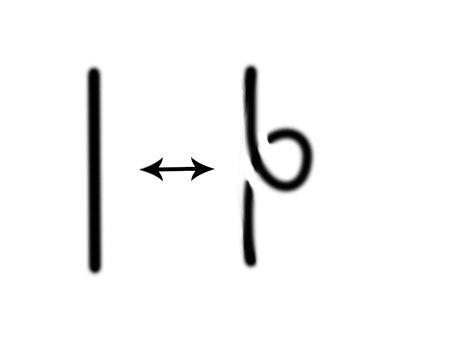
\includegraphics[width=2cm]{imagenes/movi1.png}
			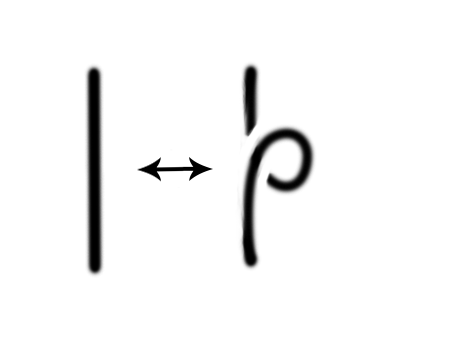
\includegraphics[width=2cm]{imagenes/movi2.png}
		\end{figure}
		\pause
		\item Segundo movimiento de Reidemeister.
		\begin{figure}[h!]
			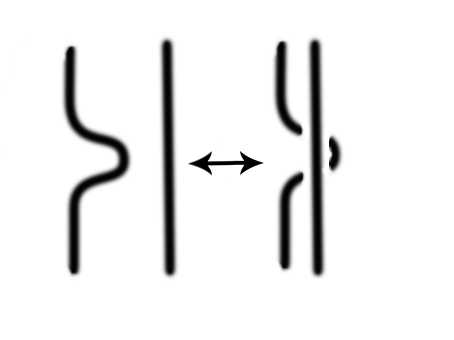
\includegraphics[width=2.8cm]{imagenes/movi3.png}
			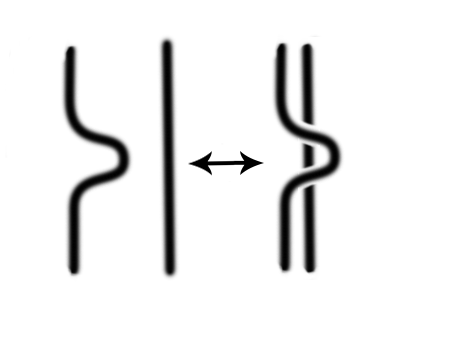
\includegraphics[width=2.8cm]{imagenes/movi4.png}
		\end{figure}
		\pause
		\item Tercer movimiento de Reidemeister. 
		\begin{figure}[h!]
			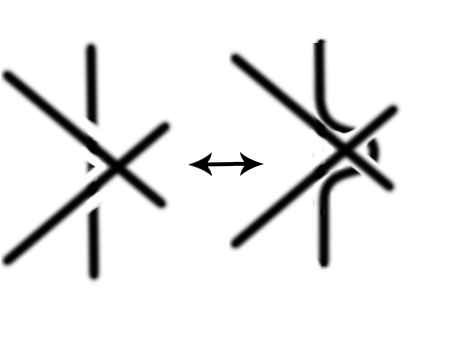
\includegraphics[width=3.2cm]{imagenes/movi5.png}
			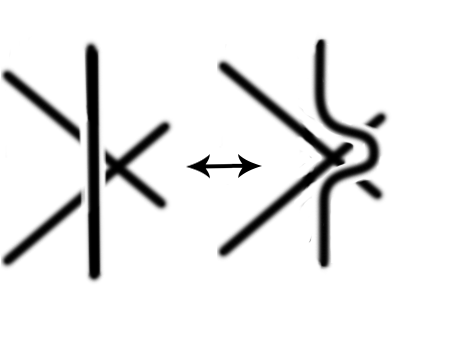
\includegraphics[width=3.2cm]{imagenes/movi6.png}
		\end{figure}
	\end{itemize}
\end{frame}

\begin{frame}{Invariantes de nudos.}
	\begin{block}{Invariante de nudo (o enlace)}
		Propiedad que no cambia cuando el nudo sufre deformaciones en el espacio.
	\end{block}
	Algunos invariantes básicos:
	\begin{itemize}
		\item Número de componentes.
		\item Crossing number. 
		\item Unknotting number. 
		\item Tricolorabilidad.
		\item Polinomio de Alexander. 
	\end{itemize}
\end{frame}

\begin{frame}{Notación de nudos.}
\textbf{ Notación de Dowker. }
	\begin{exampleblock}{(1,-4), (3,-6) , (5,2)$  \rightarrow $ -4 -6 2}
	\begin{figure}[h!]
		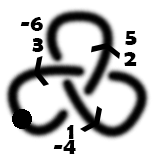
\includegraphics[width=2cm]{imagenes/3fcon2dow.png}
	\end{figure}
	\end{exampleblock}
	
\textbf{ Notación de Gauss. }
	\begin{exampleblock}{-1 2 -3 1 -2 3}
		\begin{figure}[h!]
			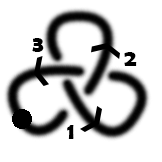
\includegraphics[width=2cm]{imagenes/3fcon2gaus.png} 
		\end{figure}
	\end{exampleblock}

\end{frame}

\begin{frame}{Conexiones con teorías - Teoría de grafos.}
\textbf{Grafo}: par $ (V,A) $ de conjuntos, junto con la aplicación 
\begin{center}
	$  \gamma :A \rightarrow$ \{\{$u,v$\} / $u,v \in V$\}  
\end{center}

\begin{exampleblock}{De proyección a grafo. }
	\begin{figure}[h!]
		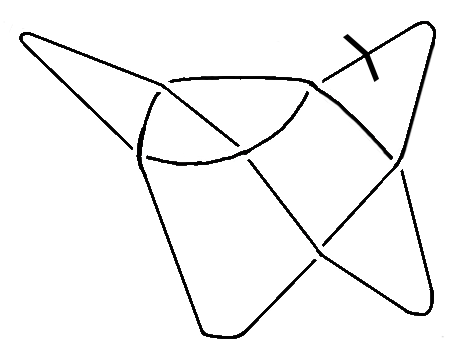
\includegraphics[width=2.5cm]{imagenes/pgrafo3.png}
		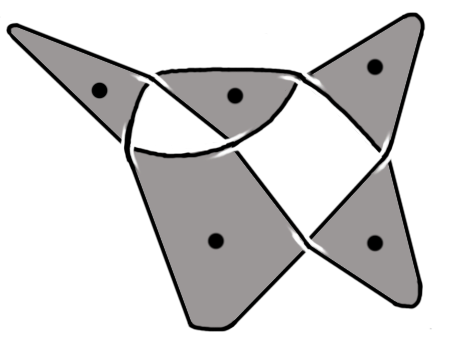
\includegraphics[width=2.5cm]{imagenes/pgrafo2.png}
		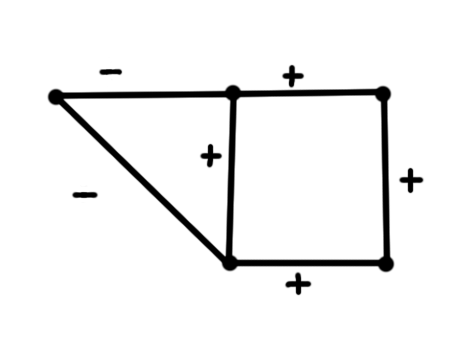
\includegraphics[width=2.5cm]{imagenes/pgrafo1.png}
	\end{figure}
\end{exampleblock}
\begin{exampleblock}{De grafo a proyección. }
	\begin{figure}[h!]
		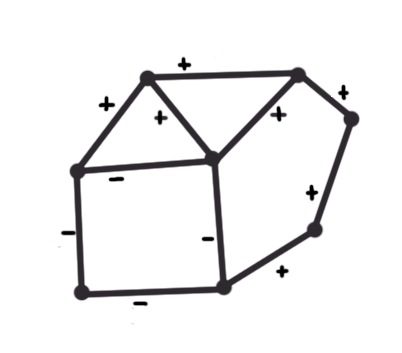
\includegraphics[width=2.5cm]{imagenes/grafo1.png}
		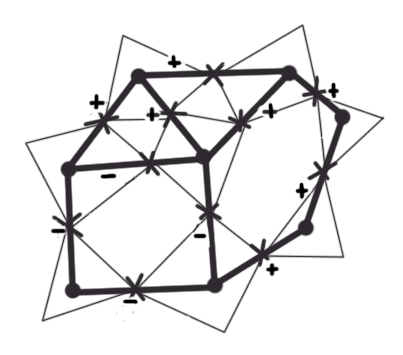
\includegraphics[width=2.5cm]{imagenes/grafo2.png}
		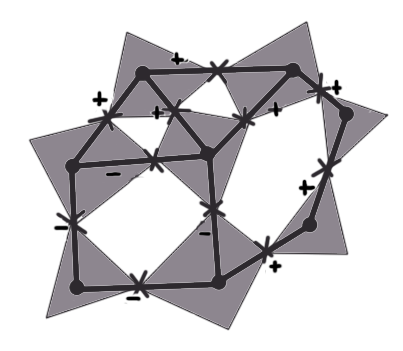
\includegraphics[width=2.5cm]{imagenes/grafo3.png}
		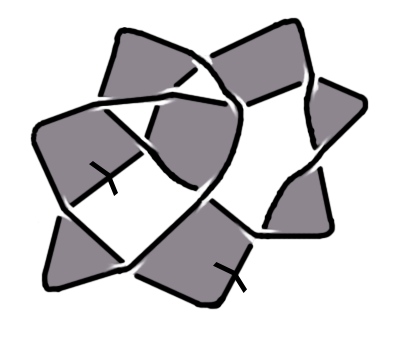
\includegraphics[width=2.5cm]{imagenes/grafo4.png}
	\end{figure}
\end{exampleblock}
\end{frame}

\begin{frame}{Conexiones con teorías - Teoría de trenzas.}
\textbf{Trenza:} Conjunto de $n$ cadenas que son atadas a un tope imaginario arriba y abajo.
\begin{exampleblock}{De trenza a nudo. }
	\begin{figure}[h!]
		
\includegraphics[width=1cm]{imagenes/t2pro.png}
		
\includegraphics[width=1cm]{imagenes/t2probien.png}
	\end{figure}
\end{exampleblock}
\begin{exampleblock}{De nudo a trenza. }
	\begin{alertblock}{Teorema de Alexander. }
		 Todo nudo puede ser representado como una trenza cerrada.
	\end{alertblock}
	\end{exampleblock}
\end{frame}


\section{Teoría de trenzas.}
\begin{frame}{Definición de trenza (I).}
\begin{alertblock}{\textbf{Trenza}}
Sea $\mathds{D} = \{(x,y,z) / 0 \leq x,y,z \leq 1\}$.\\
Situamos $A_{i}$ y $B_{i}$ puntos en las caras superior e inferior:\\
$A_{1}=(\frac{1}{2},\frac{1}{n+1},1)$, $A_{2}=(\frac{1}{2},\frac{2}{n+1},1)$,...,$A_{n}=(\frac{1}{2},\frac{n}{n+1},1)$, \\ $B_{1}=(\frac{1}{2},\frac{1}{n+1},0)$, $B_{2}=(\frac{1}{2},\frac{2}{n+1},0)$,...,$B_{n}=(\frac{1}{2},\frac{n}{n+1},0)$.\\
Unimos cada $A_{i}$ con cierto $B_{k}$ con arcos poligonales simples $d_{i}$ tal que:
\begin{enumerate}
	\item $ d_{1}, d_{2},...,d_{n} $ sean disjuntos.
	\item Los arcos $ d_{i} $ no pueden conectar puntos $A_{i}$ o $B_{i}$ entre sí.
	\item Al cortar por planos horizontales, cada arco toca en un sólo punto al plano. 
\end{enumerate}
\textbf{Cadena}: cada arco poligonal.
\textbf{Trenza}: conjunto de las n-cadenas.
\end{alertblock}
\end{frame}

\begin{frame}{Definición de trenza (II).}
\begin{figure}[h!]
	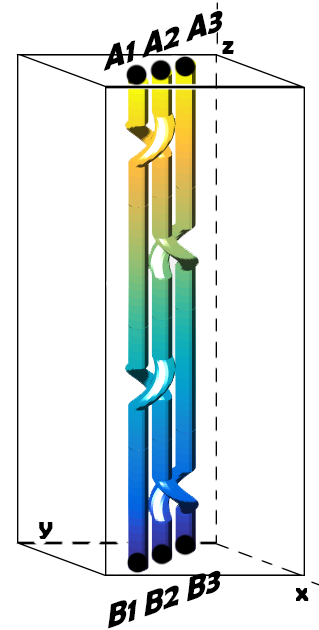
\includegraphics[width=2.5cm]{imagenes/t2cubo.png}
\end{figure}
\begin{alertblock}{$\mathscr{B}_{n}$:}
	Conjunto de todas las trenzas de n cadenas.
\end{alertblock}
\end{frame}

\begin{frame}{Equivalencia y proyección de trenzas (I). }
	\textbf{Movimiento elemental}: operación $ \Omega $ que intercambia el segmento AB por los segmentos AC $ \cup $ CB (y su inversa).
	\begin{figure}[h!]
		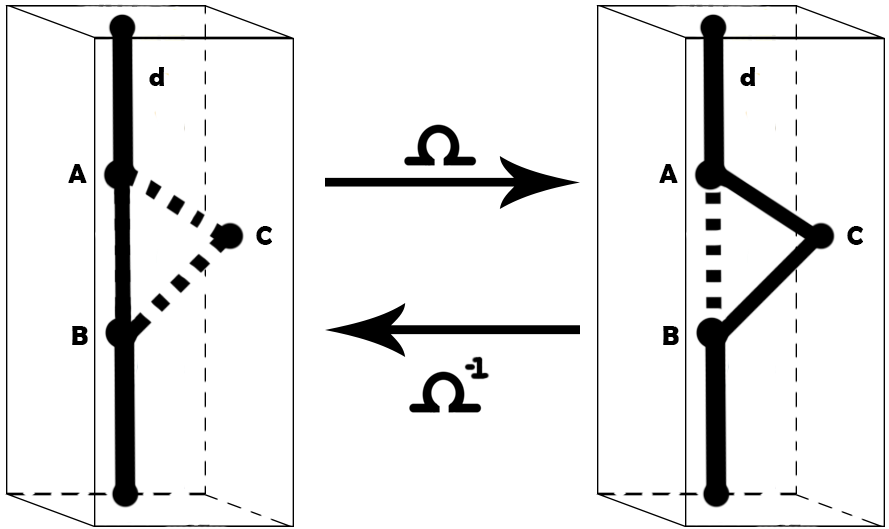
\includegraphics[width=4.5cm]{imagenes/elemental.png}
	\end{figure}

	Dos trenzas son equivalentes ($\beta \sim \beta'$) si existe una cadena finita de trenzas
		$ \beta = \beta_{0} \rightarrow \beta_{1} \rightarrow ... \rightarrow \beta_{m}=\beta'$
	
	\begin{alertblock}{${B}_{n}$:}
		Conjunto de todas las trenzas de n cadenas no equivalentes entre sí. \\
		${B}_{n}$ = $\mathscr{B}_{n}$/$ \sim $.\\
    \end{alertblock}
\end{frame}

\begin{frame}{Equivalencia y proyección de trenzas (II). }
	Proyectando visualizaremos las cadenas como curvas poligonales
	simples sobre el plano-yz.
	\begin{figure}[h!]
		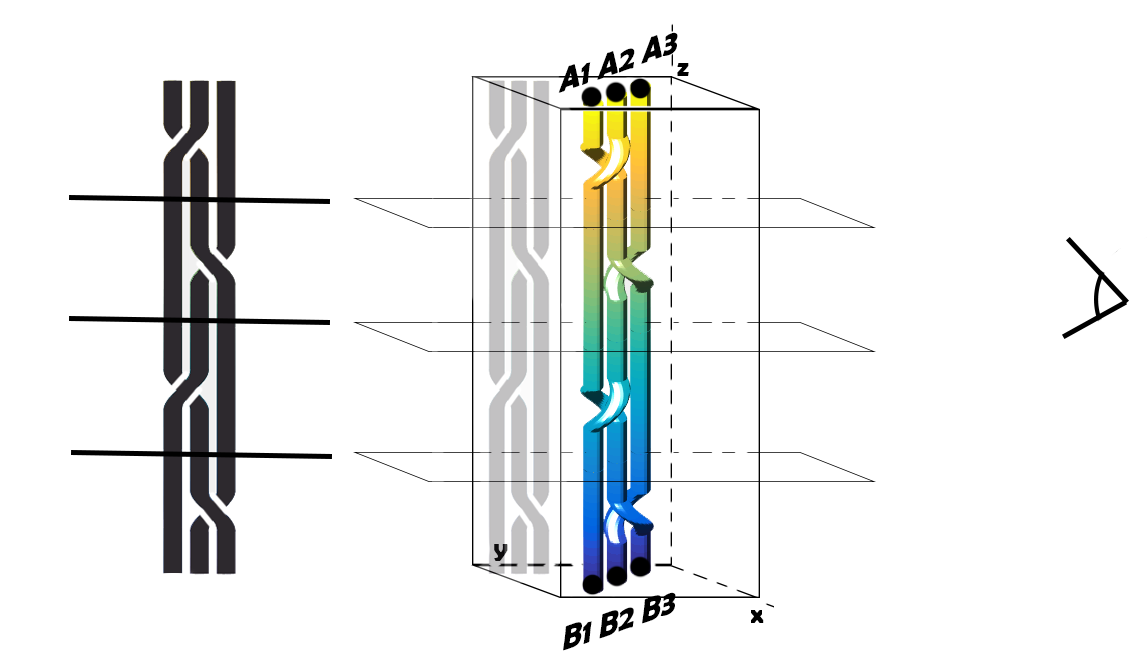
\includegraphics[width=9cm]{imagenes/pers.png}
	\end{figure}
\end{frame}

\begin{frame}{Notación de trenzas (I).}
	Consideramos la proyección de una trenza. \\
	Seleccionamos los segmentos de cadenas que producen la intersección en la proyección. Supongamos que unen las posiciones posiciones $i$ con la $i+1$ y las posiciones $i+1$ con la $i$.
	El intercambio de posiciones produce un \textbf{cruce}:
	\begin{itemize}
		\item Cruce negativo ($\sigma_{i}^{-1}$): El segmento que parte de la posición $i$ cruza por delante al segmento que inicialmente parte en la posición $i+1$.
		\item Cruce positivo ($\sigma_{i}^{+1}$): El segmento que parte de la posición $i$ cruza por detrás al segmento que inicialmente parte en la posición $i+1$.
	\end{itemize}
	\begin{figure}[h!]
		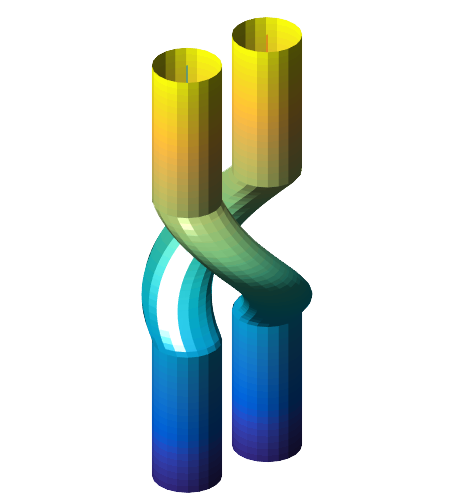
\includegraphics[width=1.8cm]{imagenes/t5.png}
	    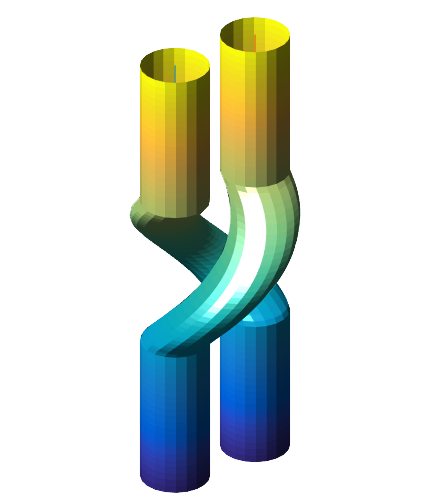
\includegraphics[width=1.8cm]{imagenes/t6.png}
	\end{figure}

\end{frame}

\begin{frame}{Grupo no abeliano.}
	Sean las trenzas $\beta$, $\beta' \in \mathscr{B}_{n}$.\\
	\textbf{Trenza producto $\beta \beta'$}: n-trenza creada uniendo los extremos finales de las cadenas de $\beta$ con los extremos iniciales de $\beta'$.\\
	\begin{figure}[h!]
		
\includegraphics[width=3cm]{imagenes/1c1.png}
		
\includegraphics[width=3cm]{imagenes/1c2.png}
		
\includegraphics[width=2.5cm]{imagenes/1c3.png} 
	\end{figure}
	\begin{alertblock}{Teorema}
		El conjunto ${B}_{n}$, dotado del producto de trenzas, es un grupo.
	\end{alertblock}
\end{frame}

\begin{frame}{Notación de trenzas (II).}
	\textbf{Palabra:} Secuencia de cruces de la trenza.
		\begin{figure}[h!]
			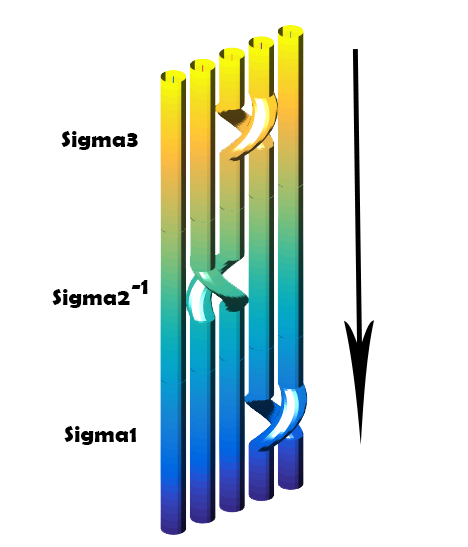
\includegraphics[width=4.2cm]{imagenes/t7.png}
			\caption{Trenza $\sigma3\sigma2^{-1}\sigma4$.}
		\end{figure}
	\textbf{\textbf{n-trenza trivial} ($1_{n}.$)}: n-trenza que no realiza ningún cruce.\\
\end{frame}


\begin{frame}{Equivalencia de trenzas. }
	Dos palabras serán equivalentes $ \leftrightarrow $ podemos pasar de una palabra a otra mediante un secuencia de estos tres movimientos:		\begin{figure}[h!]
		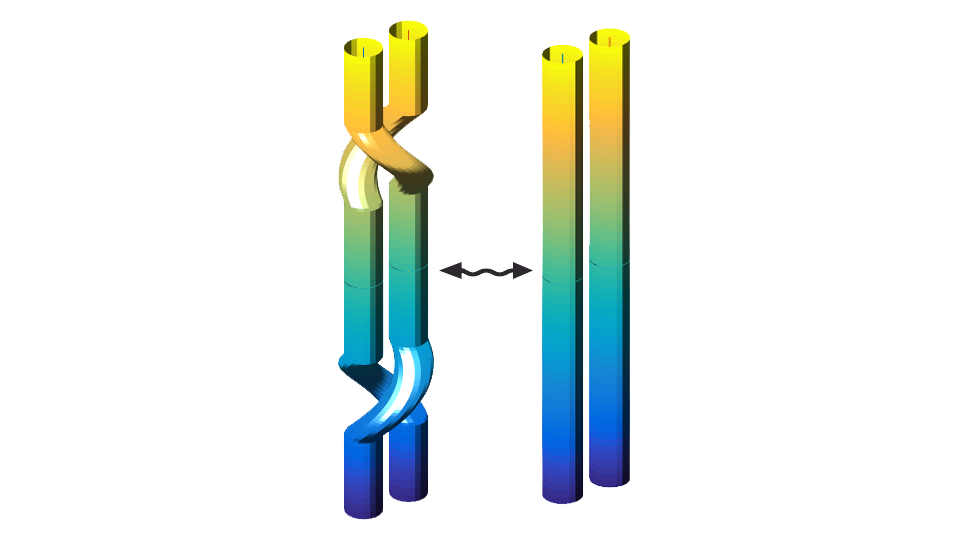
\includegraphics[width=4cm]{imagenes/M1.png}
		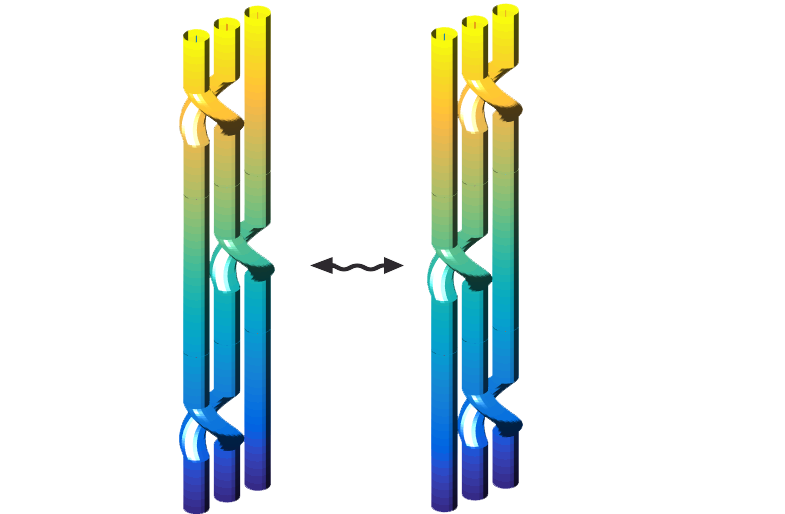
\includegraphics[width=4cm]{imagenes/M2.png}
		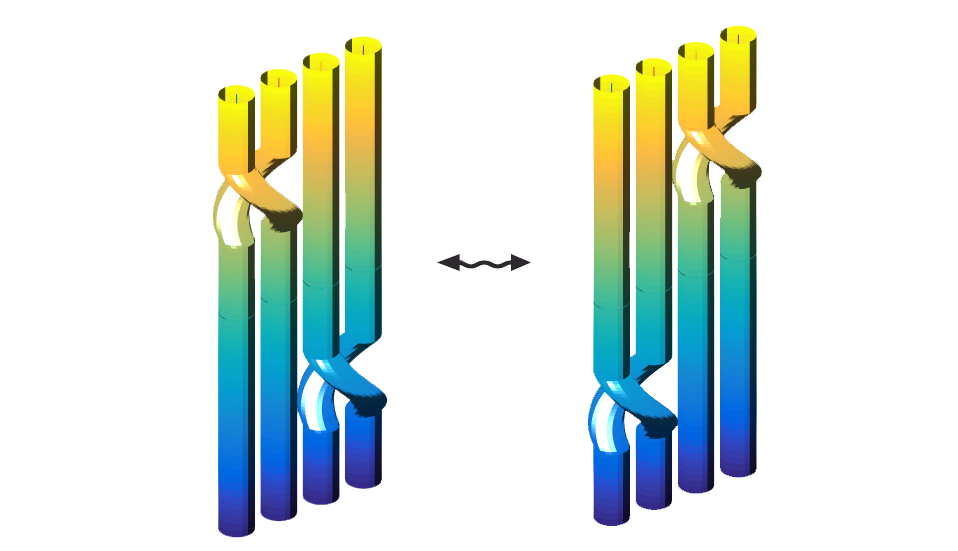
\includegraphics[width=4cm]{imagenes/M3.png}
	\end{figure}
	\begin{alertblock}{Teorema.}
			Bajo las siguientes relaciones, se tiene la igualdad final.
			\begin{enumerate}
				\item $ \sigma_{i+1}\sigma_{i}\sigma_{i+1} =\sigma_{i}\sigma_{i+1}\sigma_{i} $ siendo $i=2,..,n-2 $ \label{rel1}
				\item $ \sigma_{i}\sigma_{j}=\sigma_{j}\sigma_{i} $ siendo $1 \le i < j \le n-1 $, $j-i \geq 2$	 \label{rel2}   	
			\end{enumerate}
			\begin{center}
				$B_{n} = <\sigma1, \sigma2,..,\sigma_{n-1} /$ las relaciones \ref{rel1} y \ref{rel2} se verifican$>$
			\end{center}
	\end{alertblock}

\end{frame}

\begin{frame}{Equivalencia de trenzas cerradas - Makov equivalentes.}
    \textbf{Trenzas Markov-equivalentes}: cierres producen el mismo enlace. \\
	
	\begin{alertblock}{Teorema de Markov.}
		Dos trenzas son Markov-equivalentes $ \leftrightarrow $ podemos pasar de una trenza a otra mediante una secuencia de las tres operaciones anteriores y los movimientos de Markov (conjugación y estabilización):
	\end{alertblock}
	\begin{figure}[h!]
		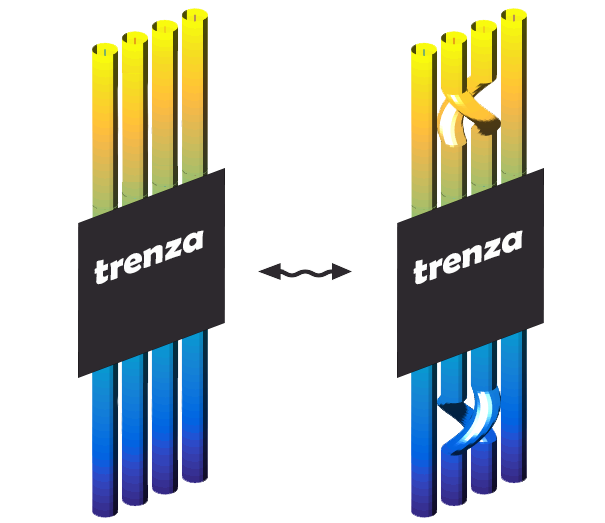
\includegraphics[width=4cm]{imagenes/M4.png}
		
\includegraphics[width=4cm]{imagenes/M5.png}
	\end{figure}
\end{frame}

\begin{frame}{Invariantes de trenzas (I).}
	\begin{block}{Invariante de trenza.}
		Propiedad que no cambia cuando la trenza sufre deformaciones.
	\end{block}
		Algunos invariantes básicos:
		\begin{itemize}
			\item Exponente.
			\item Permutación. 
			\item Polinomio de Alexander. 
		\end{itemize}
		\pause
		\begin{exampleblock}{Exponente: +1, Permutación: 1 2 4 3}
			\begin{figure}[h!]
				
\includegraphics[width=2cm]{imagenes/7c1.png}
			\end{figure}
		\end{exampleblock}
\end{frame}

\begin{frame}{Invariantes de trenzas (II) - Polinomio de Alexander.}
	\begin{block}{Matriz de Burau.}
		Sea la trenza $\beta $= $\sigma_{i_{1}}^{e_{1}} \sigma_{i_{2}}^{e_{2}} ... \sigma_{i_{m}}^{e_{m}}$ donde $e_{i} \in \{-1,1\}$, 1 $\le i_{1}, i_{2},..,i_{m} \le$ n-1. Podemos definir el homomorfismo
		\begin{center}
			$ \phi_{n} : B_{n}  \rightarrow  M(n,\mathds{Z}[t,t^{-1}])$	 
		\end{center}
		\[ \phi_{n} ( \sigma_{i}) = \begin{bmatrix}
		I_{i-1} &  &  & \\
		& 1-t & t &  \\
		& 1 & 0 &  \\
		&  &  & I_{n-i-1} \\
		\end{bmatrix}\]
	\end{block}
	\begin{alertblock}{Teorema}
		Supongamos que la trenza cerrada de $\beta$ genera el nudo K.\\
		Entonces $\exists k \in \mathds{Z}$ tal que el polinomio ($ \pm $ $ t^{k} )det[\phi_{n}(\beta)$ - $ I_{n} $$ ]_{1,1} $ es un invariante de K. (Se conoce como polinomio de Alexander, $ \triangle_{k} $(t)).
	\end{alertblock}
\end{frame}

\begin{frame}{Problema de las palabras.}
	\begin{block}{\textbf{Problema de las palabras del grupo de las trenzas:}}
		Dadas dos palabras de trenzas $\beta1, \beta2 \in B_{n}$ tratamos de encontrar algún método que nos permita confirmar si son o no equivalentes. \\
	\end{block}
	\begin{itemize}
		\item El problema de las palabras se puede reducir a distinguir si una palabra es equivalente o no a la palabra vacía.
		\item Usamos el método de Patrick Dehornoy. 
	\end{itemize}
	
\end{frame}

\section{Toxtren.}
\begin{frame}
	Software disponible para trabajar con nudos y/o trenzas:
	\begin{itemize}
		\item braidlab
		\item knotilus
		\item braid program
	\end{itemize}
	\textbf{Problemas: } Visualización, documentación, no intuitivos...\\
	\textbf{Solución: }\emph{Toxtren.}
\end{frame}

\begin{frame}{Toxtren.}
	\begin{figure}[h!]
		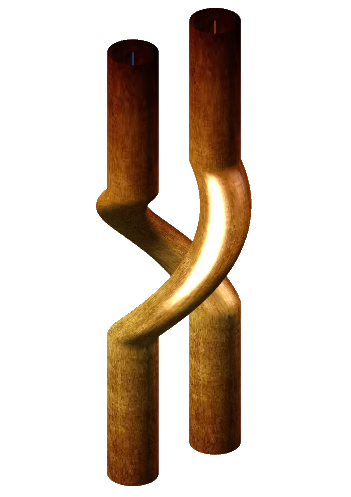
\includegraphics[width=1cm]{imagenes/im.png}
	\end{figure}
     \begin{itemize}
     	\item Toolbox creado en Matlab R2005a.
     	\item Instalación muy simple mediante toxtren.mltbx.
     	\item Diseño orientado a objetos. 
     	\item Documentación mediante help o mediante Supplemental Software. 
     \end{itemize}
     \pause
     \begin{figure}[h!]
     	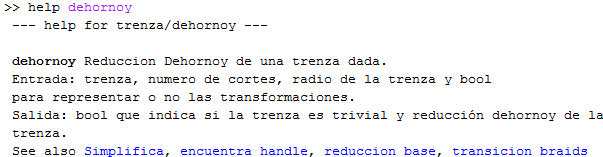
\includegraphics[width=11cm]{imagenes/help.png}
     \end{figure}
\end{frame}

\begin{frame}
	\begin{figure}[h!]
		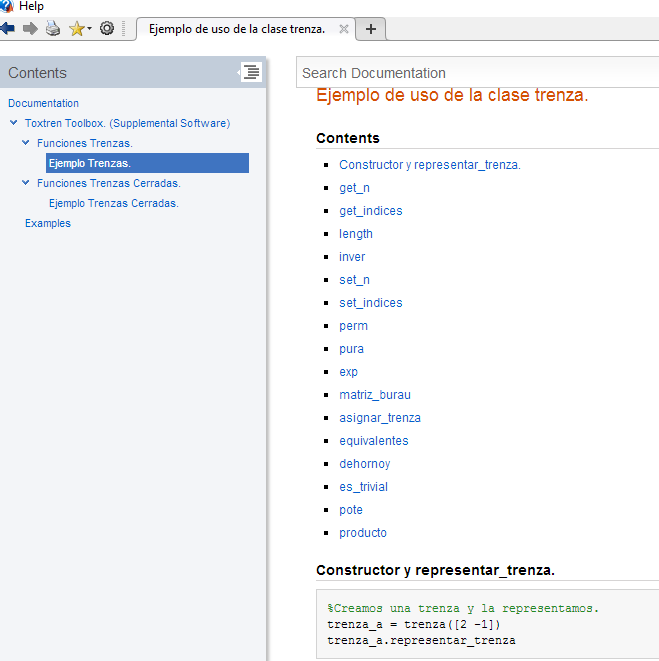
\includegraphics[width=8.5cm]{imagenes/docu.png}
	\end{figure}
\end{frame}

\begin{frame}
\begin{center}
    \includemedia[
	width=0.6\linewidth,height=0.6\linewidth,
	activate=pageopen,
	transparent,
	addresource=pruebagrab3.mp4,
	flashvars={
		source=pruebagrab3.mp4     % same path as in addresource!
	}
	]{}{VPlayer9.swf}
\end{center}
\end{frame}

\end{document}